% Adapted from ne630_problems/lesson_18/statement.tex and PWR_UnitCell.ipynb
% at commit e1fba66.
% The source CSV's P/D=2.5 epsilon value (1.157) is inconsistent with both
% neighboring values and its own k=eta*f*p*epsilon product; the plotted data
% use the product-consistent value 1.0892 and preserve all other source rows.

\noindent{\bf Problem 1.}

Modify the OpenMC PWR pin-cell model to use the parameters from Homework 17,
Problem 1, and report the four factors, $k_\infty$, and $\varsigma$.

\begin{adaptedsolution}
The source notebook uses 300 K materials, $r_f=0.5~\mathrm{cm}$,
$P=1.535~\mathrm{cm}$, 3\% enrichment, and no cladding. Its tallies give
\[
\begin{array}{c|c}
\text{quantity} & \text{OpenMC estimate}\\ \hline
\eta & 1.83231\\
f & 0.905673\\
p & 0.739180\\
\epsilon & 1.157901\\
k_\infty & 1.42033\\
\varsigma & 1.19211
\end{array}
\]
The product check gives
\[
(1.83231)(0.905673)(0.739180)(1.157901)=1.42033,
\]
consistent with the reported $k_\infty$. Relative to Homework 17, the largest
change is in $p$: $0.739$ from OpenMC versus $0.837$ from the approximate
resonance-integral model. The more explicit treatment of resonance absorption
therefore explains most of the reduction in $k_\infty$.
\end{adaptedsolution}

\newpage
\noindent{\bf Problem 2.}

At $T_f=1200~\mathrm{K}$, $T_m=600~\mathrm{K}$, and $P=15.5~\mathrm{MPa}$,
compute the four factors and $k_\infty$ over $1.1\le P/D\le3.0$.

\begin{adaptedsolution}
The source notebook results are reproduced in
Figs.~\ref{fig:hw18-koo} and \ref{fig:hw18-four-factors}.

\begin{figure}[H]
\centering
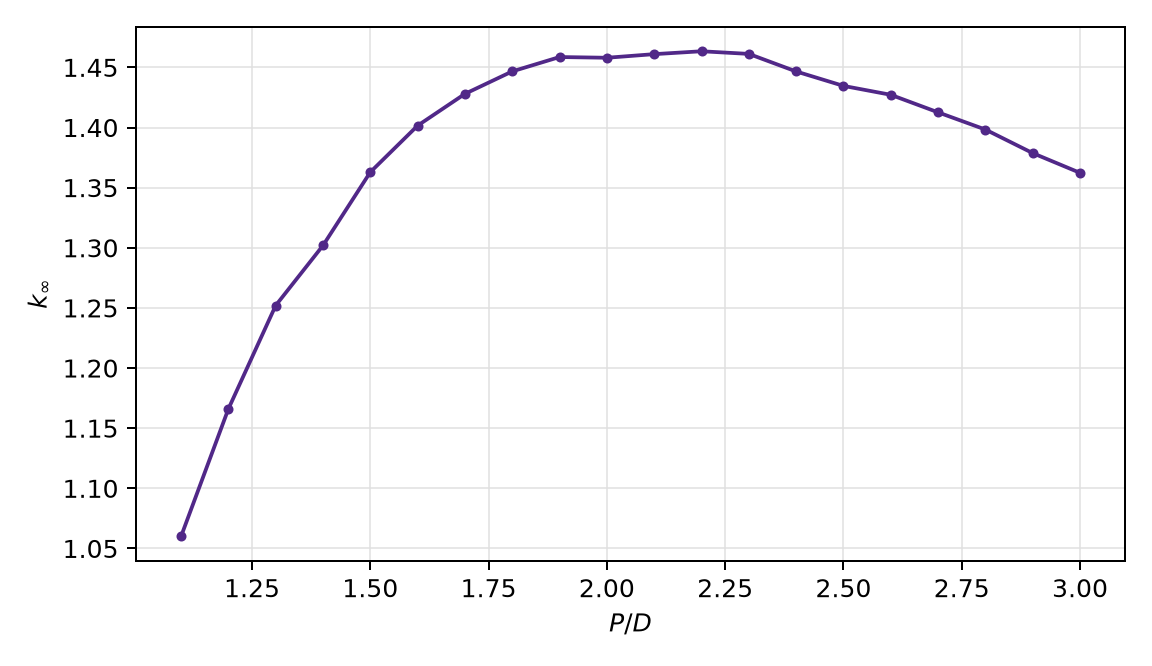
\includegraphics[width=0.68\textwidth]{hw18_koo.png}
\caption{$k_\infty$ versus $P/D$. The sampled maximum is approximately
$1.463$ at $P/D\approx2.2$.}
\label{fig:hw18-koo}
\end{figure}

\begin{figure}[H]
\centering
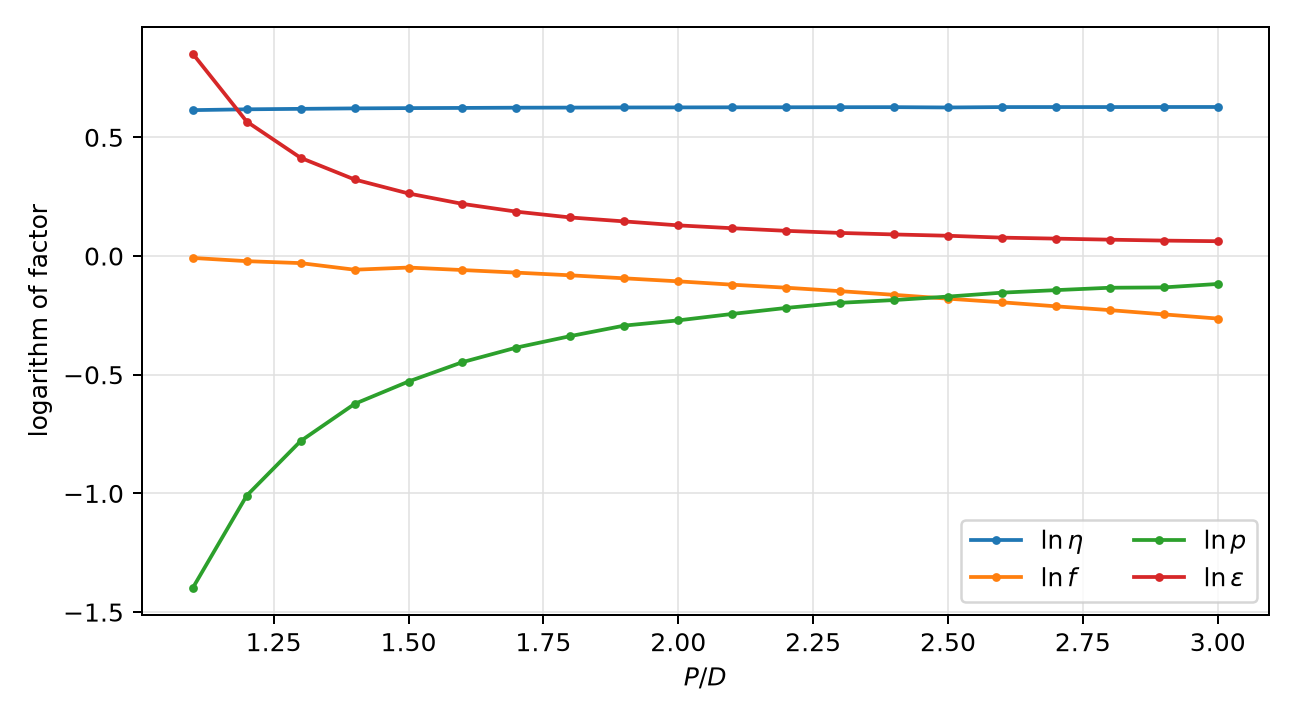
\includegraphics[width=0.86\textwidth]{hw18_log_four_factors.png}
\caption{Logarithms of the four factors versus $P/D$. Their sum is
$\ln k_\infty$.}
\label{fig:hw18-four-factors}
\end{figure}

The trend has the expected competition. Increasing moderator initially raises
$p$ strongly, while $f$ falls as a larger share of thermal absorptions occurs
outside the fuel. Their balance produces a broad optimum near $P/D=2.2$.
$\eta$ changes little. At the smallest pitches, $\epsilon$ rises sharply
because the spectrum is much harder; this is a spectral effect and is visible
as the steep positive $\ln\epsilon$ contribution. For $P/D\gtrsim1.5$, the
usual $p$--$f$ tradeoff dominates.
\end{adaptedsolution}

\newpage
\noindent{\bf Problem 3 [Bonus].}

Construct the specified hexagonal SFR cell, find the PuO$_2$ fraction giving
$k_\infty=1.1$, and compare the regional spectra with the approximation in
FNRP Eq.~(4.8).

\begin{draftsolution}
This source problem did not include a numerical legacy solution. A complete,
reproducible solution should use the following procedure.

Let $x$ be the PuO$_2$ volume fraction within the fuel. Construct separate
natural-UO$_2$ and ${}^{239}$PuO$_2$ materials at
$10.5~\mathrm{g\,cm^{-3}}$, and create the fuel with
\texttt{openmc.Material.mix\_materials(..., percent\_type="vo")}. Preserve
the example notebook's fuel radius, cladding radius, hexagonal pitch,
temperatures, and boundary conditions.

For each trial $x$, run the same adequately converged eigenvalue calculation
and retain both $k_\infty(x)$ and its reported standard deviation. First find
a bracket $[x_L,x_U]$ for which
\[
[k_\infty(x_L)-1.1][k_\infty(x_U)-1.1]<0.
\]
Use bisection (or a safeguarded secant method) until the bracket width meets a
declared composition tolerance and $|k_\infty-1.1|$ is no larger than a few
Monte Carlo standard deviations. Report the final bracket, not spurious
digits from one noisy run. Verify the final composition with an independent
random seed.

Add identical energy filters to cell-flux tallies for fuel, cladding, and
coolant. Divide each group tally by its region volume and energy-bin width
before comparing spectra. The expected result is that the three normalized
fast spectra have broadly similar shapes because the fast-neutron mean free
path is long relative to one pin cell. That observation supports the
homogenized, common-spectrum volume averaging used in FNRP Eq.~(4.8). Any
visible resonance-scale or near-interface differences delimit the
approximation: they show what is lost when local spectra are replaced by one
cell-averaged fast spectrum.

The numerical value of $x$ remains a run-dependent grading reference until
the exact example-notebook version, cross-section library, histories, and
random seed are frozen with the assignment.
\end{draftsolution}
